\section{Experimental Results}\label{sec:exp}
In this section we present the results of our experimental evaluation of
\algonameapx. 

\para{Goals} First, we show that for a given sample $\Sample$, \algonameapx
converges quickly to a schedule $\sched^*$ that minimizes $\cost_\theta(\sched,
\Sample)$ (see Thm.~\ref{thm:optimal}). In particular, our experiments
illustrate that the sequence $\cost_\theta(\sched^1,\Sample), \cost_\theta(\sched^2, \Sample),
\ldots$ is descending and converges after few iterations. Next, we compare the
output schedule of \algonameapx to three other schedules: (i) uniform schedules,
(ii) proportional to out-degrees, and (iii) proportional to in-degrees.
Specifically, we compute the costs of these schedules according to a sample
$\Sample$ that satisfies the condition in Lemma~\ref{lem:chernoffcost} and
compare them.
%Next, for further investigation, for each generated sequence of
%$\sched^1,\sched^2,\ldots$ according to a sample $\Sample$, we compute the cost
%of $\sched^i$'s according to another test sample $\Sample'$, and see that the
%sequence $\cost_\theta(\sched^1,\Sample'), \cost_\theta(\sched^2,\Sample'),\ldots$ is still
%descending and converges after few steps.
Then, we demonstrate how our method can adapt itself to the changes in the
network parameters. Finally, we consider a specific example for which we know
the \emph{unique} optimal schedule, and show that for larger samples
\algonameapx outputs a schedule closer to the optimal optimal.

% Finally,  we show how one can use {\optimizer} to extract a set of nodes as a solution the the Influence-Maximization problem, and we compare it to \texttt{TIM+}\cite{??}. \texttt{TIM+} is an algorithm for Influence-Maximization problem that is based on sampling \emph{hyper-edges} (see \cite{borgs,??}) and running a greedy algorithm for submodular optimization. We see that by {\optimizer} we can obtain seeds whose influence are close to \texttt{TIM+}'s output seeds with much smaller running time.

% Next, for different samples and different number of iterations, we test the quality of the output schedule, according to a test sample $\Sample'$, i.e., we evaluate the cost of each of the schedules in the iterative method with respect to $\Sample'$, $\cost{\sched,\Sample'}$ . \ahmad{\st{Finally, we illustrate the behavior of {\optimizer} when the network parameters change.}}

\begin{table}[ht]
\centering
\resizebox{\columnwidth}{!}{
\begin{tabular}[scale=0.5]{l r r c r}
\toprule
Datasets	& \#nodes	& \#edges & $(|V_{1K}|,|V_{500}|,|V_{100}|)$ & gen. rate\\
%\hline \hline
\midrule
Enron-Email	& 36692	& 367662&(9,23,517) & 7.22\\
%\hline
Brightkite	&58228	&428156	&(2,7,399)	& 4.54\\
%\hline
%Epinion		&75879	&508837	&8	&45	&917& 12.22\\
%\hline
web-Notredame	&325729	&1497134& (43,80,1619)& 24.49\\
% \hline
web-Google	&875713	&5105039&(134,180,3546)	& 57.86\\
%\hline
%Twitter 	&81306	&1768149&43	&108	&2674& 36.44\\
%\hline
\bottomrule
\end{tabular}
}
\caption{\scriptsize The datasets, corresponding statistics, and the rate of generating new items at each step.}\label{table:datasets}
\end{table}

\para{Environment and Datasets.} We implemented \algonameapx in C++. The implementation of \algonameapx never loads the entire sample
to the main memory, which makes it very practical for running large samples on
conventional machines. The experiments were run on a Opteron 6282 SE CPU (2.6
GHz) using 12G memory. We tested our method on a number of datasets from the
SNAP repository\footnote{\url{http://snap.stanford.edu}} (see
Table~\ref{table:datasets} for details).
%\begin{itemize*}
% \item Enron-Email~\cite{klimt2004introducing}: The email communication of Enron Corporation.
% \item Brightkite~\cite{ChoML11}: A location-based online social network, where each edge represents a friendship tie.
% \item Epinion~\cite{richardson2003trust}: The trust relationships in \texttt{Epinion.com}.
%%  \item wiki-Vote~\cite{wikivote1,wikivote2}: A network between Wikipedia users where each edge shows a vote from a user for another one.
%  \item web-Notredame~\cite{notredame}: Network of ``University of Notre Dame'' where each edge represents a hyperlink from a page to another page.
% \item web-Google~\cite{webgoogle}: A dataset released by Google in 2002, where each node is a page and a directed edge represents a hyperlink between the pages.
% \item Twitter~\cite{McAuleyL12}: A combined ego network, where each edge is directed from a node to another node that it follows.
%\end{itemize*}
%\mynote[Matteo]{Do we need to introduce the datasets here? what about just reference and the Table 1?}
%\reply[Ahmad]{No, you can remove this list, we don't even need to have the
%references, the link to snap.stanford.edu is enough. Matteo}

\para{Parameters and model of propagation}
We always let the graphs be directed by replacing undirected edges with two
directed ones. Through our experiments (except Sect.~\ref{sec:example}), we
consider the Independent-Cascade (IC)~\cite{Kempe2003} as the propagation model,
assume the activity of a node (its rate of generating new items) is a function
of its out-degree (i.e., the number of neighbors influenced by that node).
Therefore, we group the nodes based on their degrees as follows:
\begin{itemize*}
 \item $V_{1K} = \{i\in V ~:~ \degree^+(i) \geq 1000\}$,
 \item $V_{500}  = \{i\in V ~:~ 500\leq \degree^+(i) < 1000\}$,
 \item $V_{100}  = \{i\in V ~:~ 100\leq \degree^+(i) < 500\}$, and
 \item $V_{0}    = \{i\in V ~:~ \degree^+(i) < 100\}$,
\end{itemize*}
where $\degree^+(i)$ is the out-degree of node $i$ (see Table~\ref{table:datasets}).
We assume each node may generate a new item, that will be propagated, at each
time based on the group the node is assigned to. In particular, we assume that
the probability of  node $i$ generating a new item, $\pi_i$, is as follows,
based on the intuition that active individuals are  likely to have more
followers/friends:
%  $\pi=(\pi_1, \ldots, \pi_n)$, where
$$
   \pi_i = \left\{
     \begin{array}{ll}
       0.1 &: i \in V_{1K}\\
       0.05 &: i \in V_{500} \\
       0.01 &: i \in V_{50} \\
       0 & : \text{otherwise} \\
     \end{array}
   \right.
$$
 In Table~\ref{table:datasets} the expected number of new items at each time
 step is given, for each dataset, in the leftmost column (\emph{rate of new
 items}). Also, for each directed edge $e=v\rightarrow w$ we associate  a probability
$p_e$ that a new item at node $v$ is propagated through this edge to node $w$ (as in IC model),
and events for different items are independent. Following the parameters
reported in the
literature~\cite{Kempe2003,Chen2009,Chen2010,jung2011irie,tang2014influence}, we
set $p_{v\rightarrow w} = \frac{1}{\degree^-(w)}$. Finally, note that for each set of nodes, $S$, this model implicitly imposes a probability $\pi(S)$, that is unknown to \algonameapx.


%As the model of propagation, we consider the Independent-Cascade
%model~\cite{Kempe2003}:  each directed edge $e=v\rightarrow w$ has a probability
%$p_e$ that a new item at node $v$ is propagated through this edge to node $w$,
%and events for different items are independent. Following the parameters
%reported in the
%literature~\cite{Kempe2003,Chen2009,Chen2010,jung2011irie,tang2014influence}, we
%set $p_{v\rightarrow w} = \frac{1}{\degree^-(w)}$.
%For every edge $e=(a,b)$ we let the activation probability $p_e$ to be $\frac{1}{\degree^-(b)}$ which is a commonly used parameter~.


%\todo[Ahmad]{Please use the ctable package for tables, they look much better.}

\subsection{Efficiency and Accuracy}
In Sect.~\ref{sec:optimize} we showed that when a run of \algonameapx converges
(according to a sample $\Sample$) the computed $c$-schedule is optimal with
respect to the sample $\Sample$ (Lemma~\ref{lem:optimal_sample}). In our first
experiment, we measure the rate of convergence and the execution time of
\algonameapx. We fix $\epsilon=0.1$, $\theta=0.75$, and consider
$c\in\{1,3,5\}$. For each dataset, we use a sample $\Sample$ that satisfies~\eqref{eq:samp_cond}, and run \algonameapx
for 30 iterations. Denote the schedule computed at round $i$ by $\sched^i$.
As shown in Figure~\ref{fig:conv}, the sequence of cost values of the schedules
$\sched^i$'s, $\cost_\theta(\sched^i,\Sample)$, converges extremely fast after few iterations.

%the sequences of cost values according to both sample $\Sample$ and the test sample $\Sample'$ are descending and converge after few steps. Also note that the cost values according to $\Sample$ and $\Sample'$ are close (in some cases almost identical), which agrees with the theoretical analysis in Section~\ref{sec:sampcomp}.

%
%Formally,
%suppose $\sched^i$ is the obtained schedule by \algonameapx, according to the
%sample $\Sample$, at the $i$-th round of iteration. An important question
%regarding the  convergence of \algonameapx according to a sample $\Sample$ is this: If $\Sample'$ is another sample (with probably larger size) is the sequence $\cost_\theta(\sched^1,\Sample'),\cost_\theta(\sched^2,\Sample'),\ldots$ still descending and converging? This is important as we have to  avoid over-fitting our schedule with the sample $\Sample$.
%
%To demonstrate the convergence of \algonameapx we sample all the sets generated during
%a time interval of length 2000, $\Sample$. For $c\in\{1,3,5\}$ the cost of each $c$-schedule during the iterative method according to $\Sample$ is shown in Figure~\ref{fig:conv}. Also, in Figure~\ref{fig:conv}, the cost of each intermediate $c$-schedule generated during the iterative method (applied to $\Sample$) is computed according to a test sample $\Sample'$ that has been obtained during a time interval of length 10000. In both cases the cost values are decreasing.
%
%
%
%As shown in Figure~\ref{fig:conv}, the sequences of cost values according to both sample $\Sample$ and the test sample $\Sample'$ are descending and converge after few steps. Also note that the cost values according to $\Sample$ and $\Sample'$ are close (in some cases almost identical), which agrees with the theoretical analysis in Section~\ref{sec:sampcomp}.
%




%However in some cases the cost values are very close (and close to the uniform schedule) so their cost is already close to the optimal cost and their plot is almost horizontal.

%  Figure~\ref{fig:conv} reports the convergence rate of runs of {XXX}  for the networks.
% We see that for all networks and sample size the process converges in less than 12 iterations.

\begin{table}[ht]
\centering
\resizebox{\columnwidth}{!}{
\begin{tabular}[scale=0.5]{l r r r}
\toprule
Datasets	& $|\Sample|$ & avg. item size & avg. iter. time (sec)\\
%\hline \hline
\midrule
Enron-Email		&97309	&12941.33  & 	204.59\\
Brightkite		&63652	&17491.08  & 	144.35\\
web-Notredame	&393348	&183.75	   &  	10.24\\
web-Google		&998038	&704.74 	   &	121.88\\
\bottomrule
\end{tabular}
}
\caption{\scriptsize Sample size, average size of items in the sample, and the running time of each iteration in \algonameapx (for $c=1$).}\label{table:time}
\end{table}


For each graph, the size of the sample $\Sample$, the average size of sets in
$\Sample$, and the average time of each iteration is given in
Table~\ref{table:time}. Note that the running time of each iteration is a
function of both sample size and sizes of the sets (informed-sets) inside the
sample.

%As shown in Figure\ref{fig:optimizer}, {\optimizer} quickly converges to (an almost) optimal schedule.
%\mynote[Ahmad]{I'm removing the results for twitter and epinion: there was a problem for these two + 4 data sets seems enough (2 directed and 2 undirected)}

\begin{figure}[htbp]
\subcaptionbox*{}{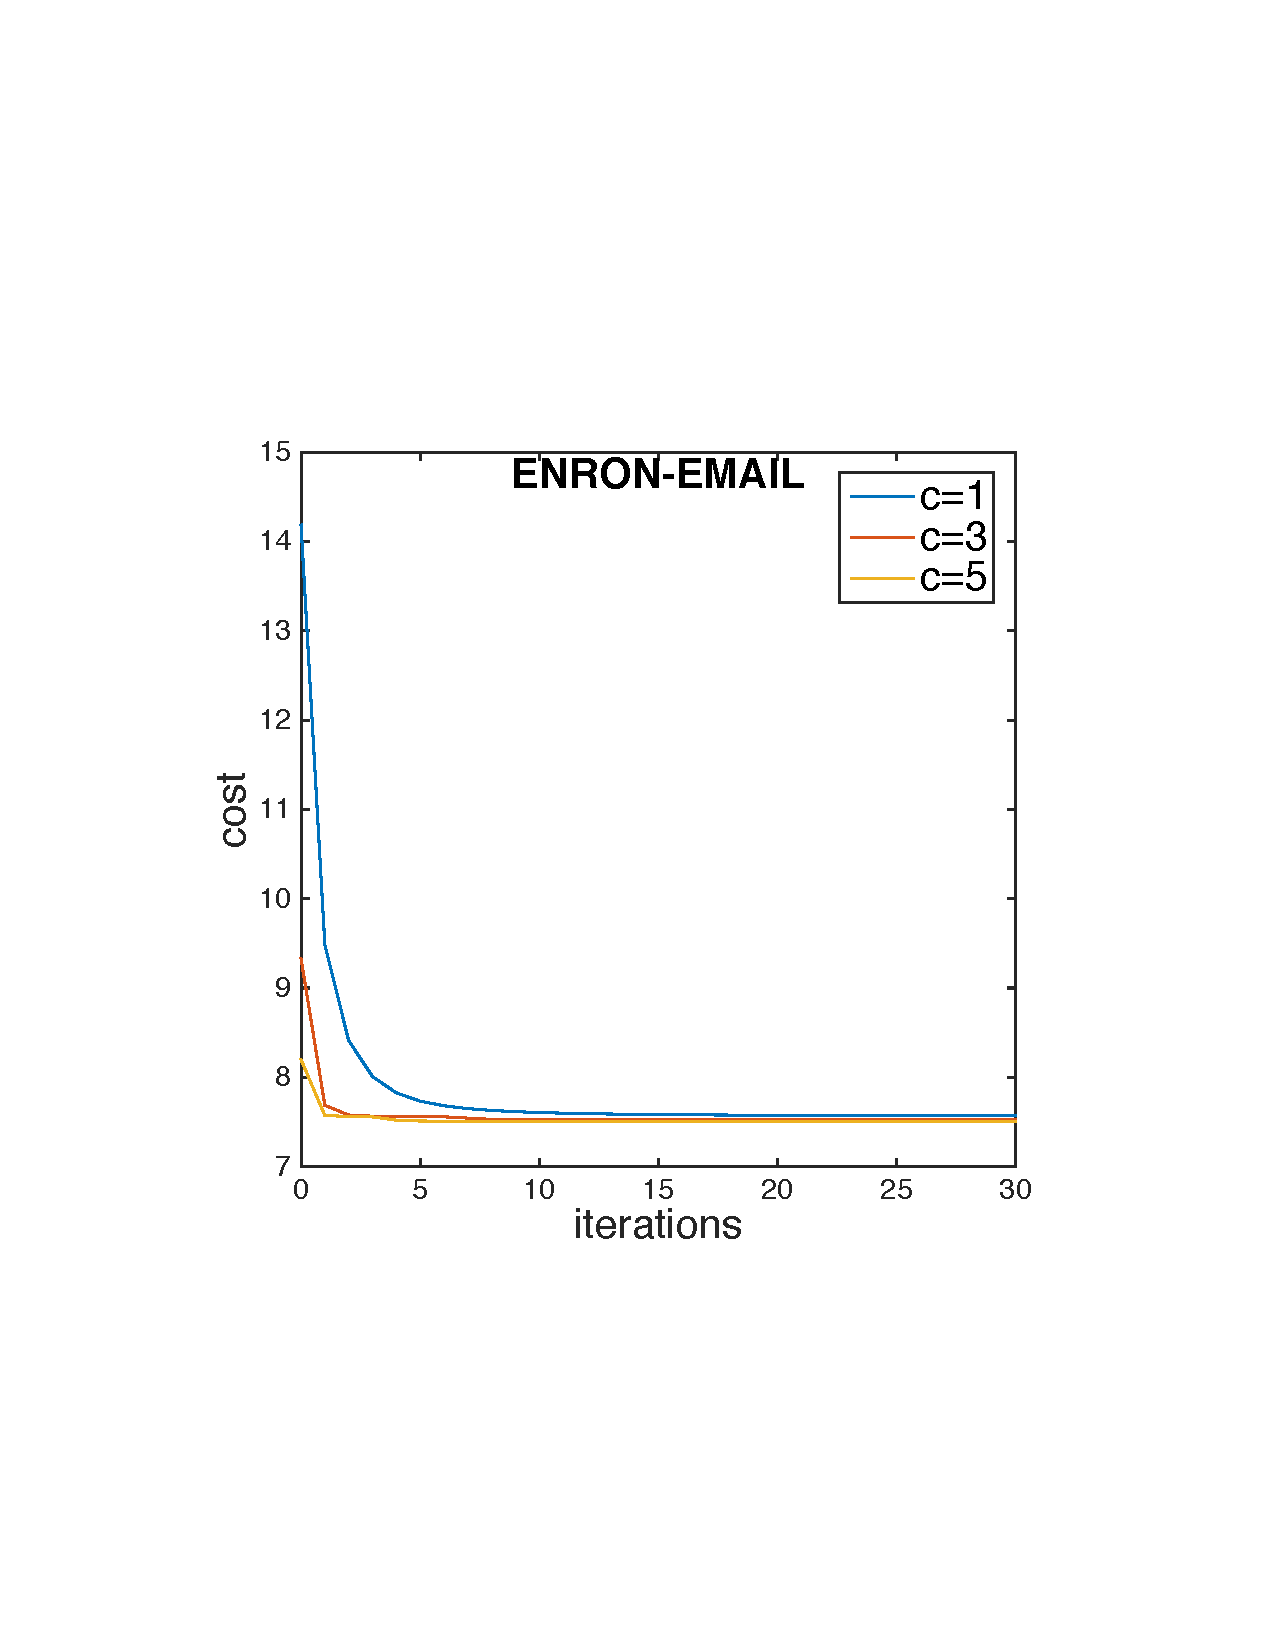
\includegraphics[width=0.49\textwidth]{figures/conv/enron-email.pdf}}
\subcaptionbox*{}{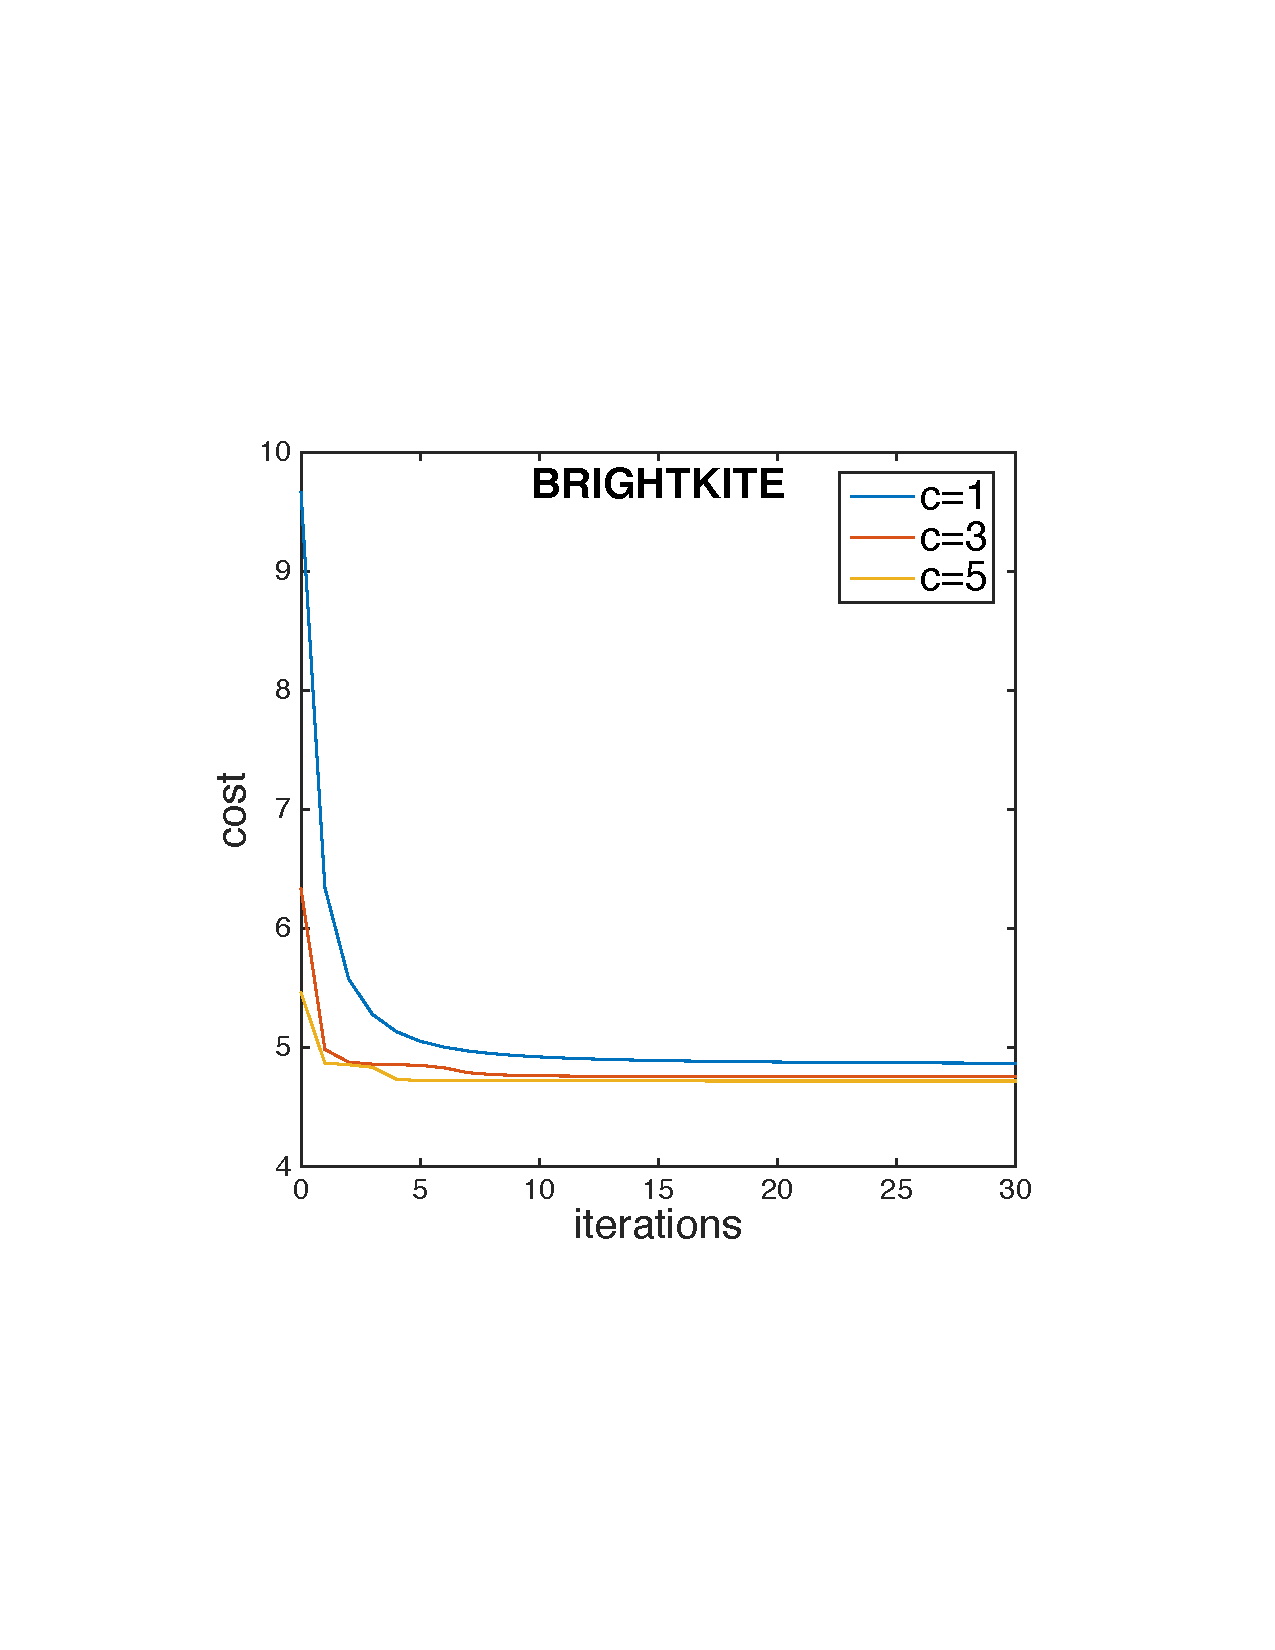
\includegraphics[width=0.49\textwidth]{figures/conv/brightkite.pdf}}
\subcaptionbox*{}{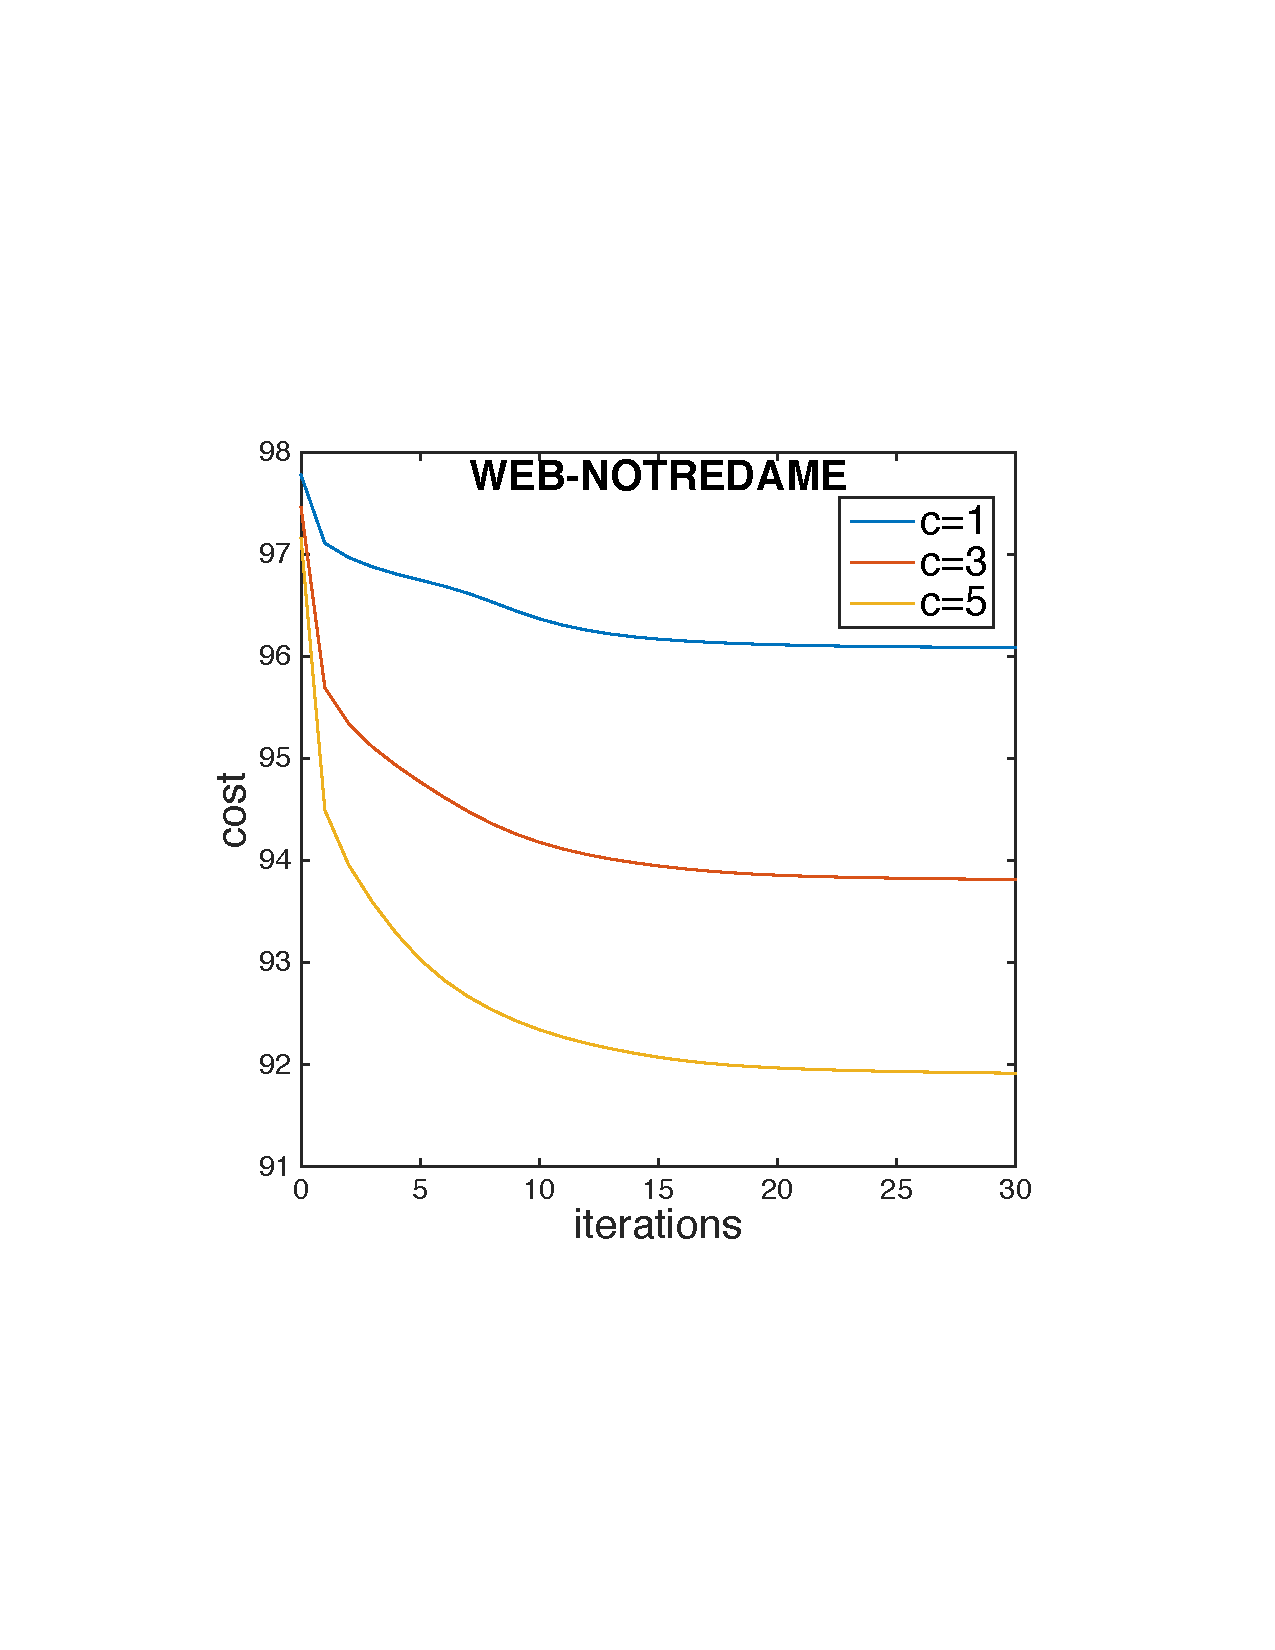
\includegraphics[width=0.49\textwidth]{figures/conv/web-notredame.pdf}}
\subcaptionbox*{}{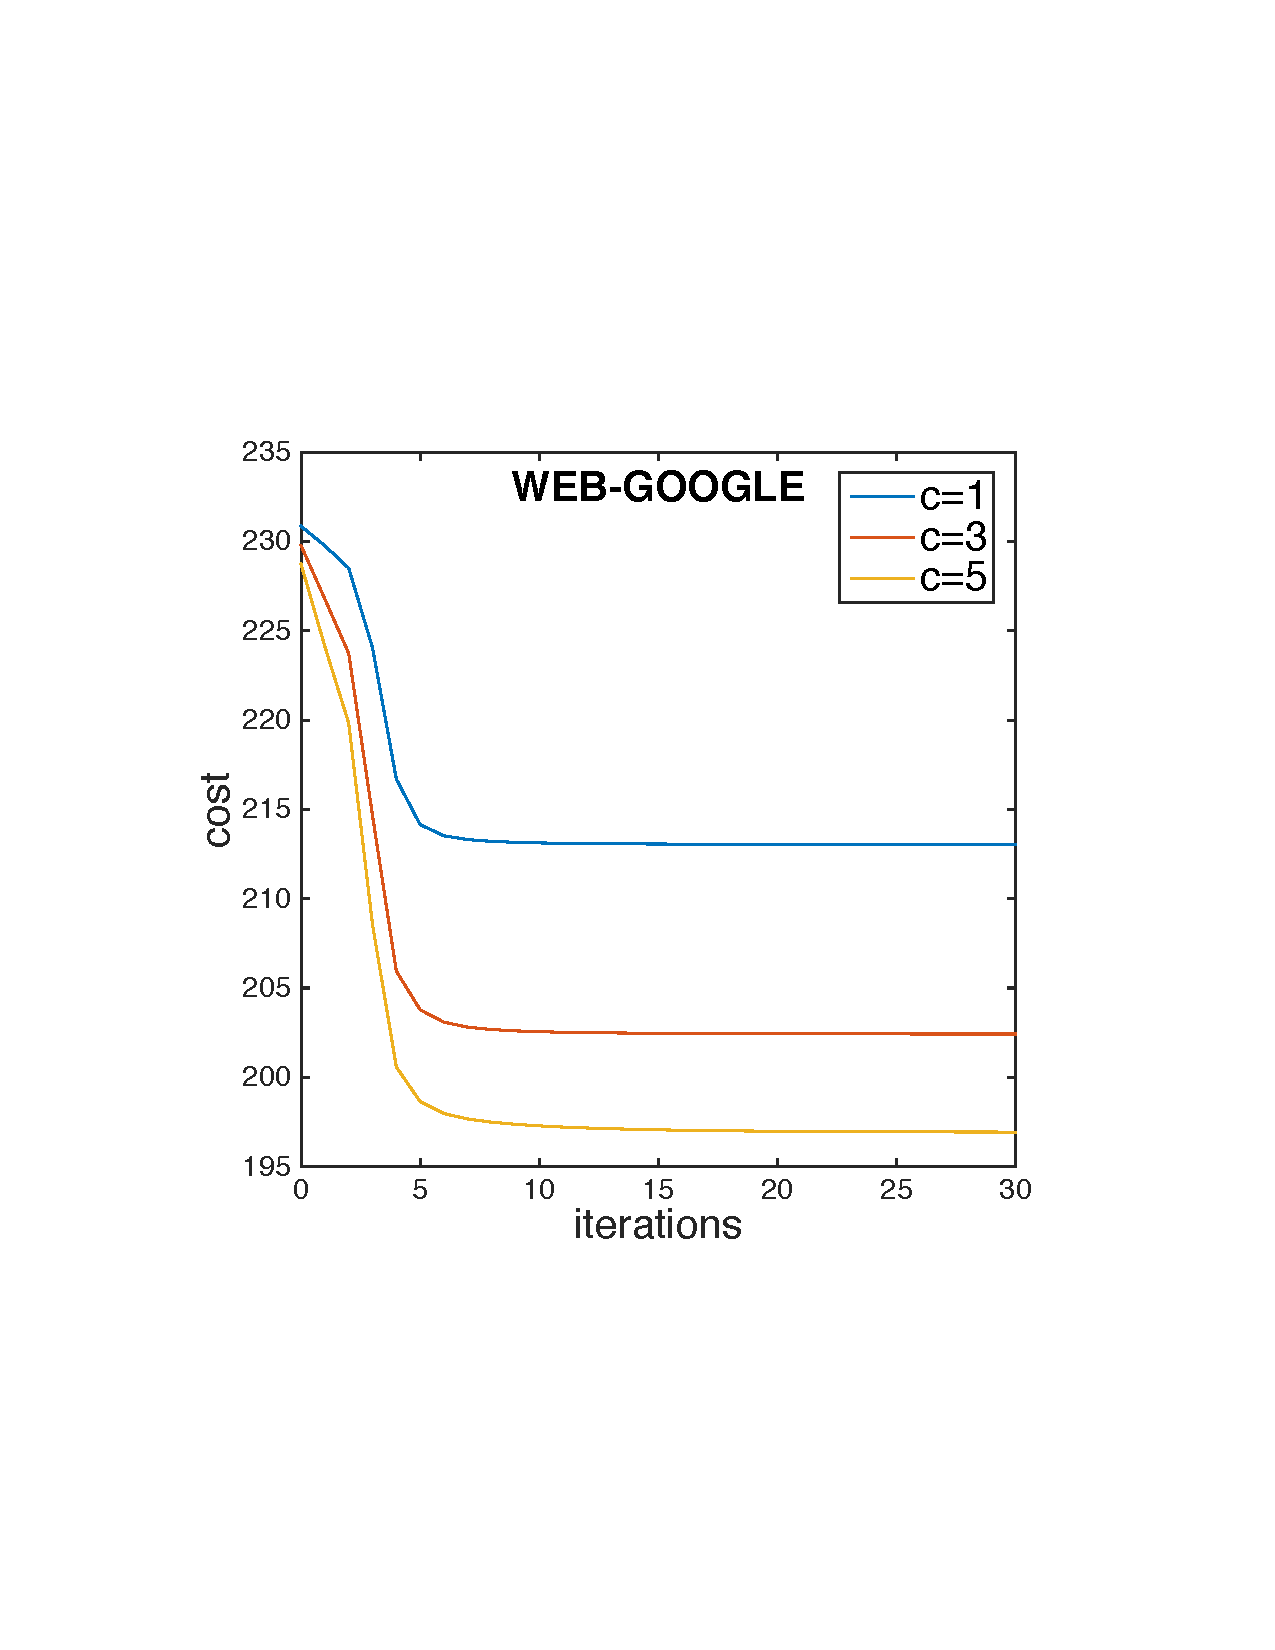
\includegraphics[width=0.49\textwidth]{figures/conv/web-google.pdf}}
\caption{\scriptsize The cost of intermediate $c$-schedules at iterations of \algonameapx  according to $\Sample$.}\label{fig:conv}
\end{figure}







Next, we extract the $1$-schedules  output by \algonameapx, and compare its cost to four other natural schedules: \texttt{unif}, \texttt{outdeg}, \texttt{indeg}, and \texttt{totdeg} that probe each node, respectively, uniformly, proportional to its out-degree, proportional to its in-degree, and proportional to number of incident edges. Note that for undirected graphs \texttt{outdeg}, \texttt{indeg}, and \texttt{totdeg} are essentially the same schedule. 

To have a fair comparison among the costs of these schedules and \algonameapx, we calculate their costs according to 10  independent samples, $\Sample_1,\ldots,\Sample_{10}$ that satisfy \eqref{eq:samp_cond}, and compute the average. The results are shown in Table~\ref{table:compare}, and show that \algonameapx outperforms the other four schedules.


%(i) \texttt{uniform} schedule, (ii) \texttt{outdeg} schedule that probes each node proportional to its out-degree, (iii) \texttt{indeg} schedule that probes each node proportional to its in-degree, and (iv) \texttt{totdeg} (note that for undirected graphs \texttt{outdegree} and \texttt{indegree} are the same). We compared the cost of these schedules according to another sample $\Sample'$ that satisfies the condition in Lemma~\ref{lem:chernoffcost}, and the results are shown in Table~\ref{table:compare}; numbers are obtained by averaging the 10 runs over 10 different sample $\Sample'$s.

\begin{table}[ht]
\centering
\resizebox{\columnwidth}{!}{
\caption{\scriptsize Comparing the costs of 5 different 1-schedules.}
\label{table:compare}
\begin{tabular}{lrrrrr}
\toprule
Dataset       & \algonameapx & \texttt{uniform} & \texttt{outdeg} & \texttt{indeg} & \texttt{totdeg} \\ 
\midrule
Enron-Email   &       7.55 & 14.16 & 9.21 & 9.21 & 9.21                  \\ 
Brightkite    &       4.85 & 9.64 & 6.14 & 6.14 & 6.14                  \\ 
web-Notredame &       96.10 & 97.78 & 97.37 & 97.43 & 97.40             \\ 
web-Google    &       213.15 & 230.88 & 230.48 & 230.47 & 230.47       \\
\bottomrule
\end{tabular}
}
\end{table}



% --------------------------------------------------
% --------------------------------------------------
% --------------------------------------------------
\subsubsection{A Test on Convergence to  Optimal Schedule}\label{sec:example}
Here, we present an example for which we know the optimal schedule, and moreover, the optimal schedule is unique. Therefore, we use this example to investigate further the convergence of \algonameapx. In particular, we would like to see how close the \algonameapx output is to the optimal schedule, regarding (i) different initial schedules, $\sched^0$ (which we let to be uniform), and (ii) samples $\Sample$'s  obtained during time intervals of different lengths.

Suppose $G=(V,E)$ is the complete graph where $V=[n]$. Let $\sys=(\family, \pi)$ for  $\family = \{S \in 2^{[n]} \mid 1 \leq|S| \leq 2\}$, and $\pi(S)=\frac{1}{|\family|}$. It is easy to see that $\cost_\theta(\sched)$ is a symmetric function, and thus, the uniform schedule is optimal. Moreover, by Corollary~\ref{corol:convexity} the uniform schedule is the only optimal schedule, since $\{v\} \in \family$ for every $v\in V$. Furthermore, we let $\theta=0.99$ to increase the sample complexity (as in Lemma~\ref{lem:chernoffcost}) and make it harder to learn the uniform/optimal schedule.

\begin{figure}[htbp]
	\subcaptionbox*{}{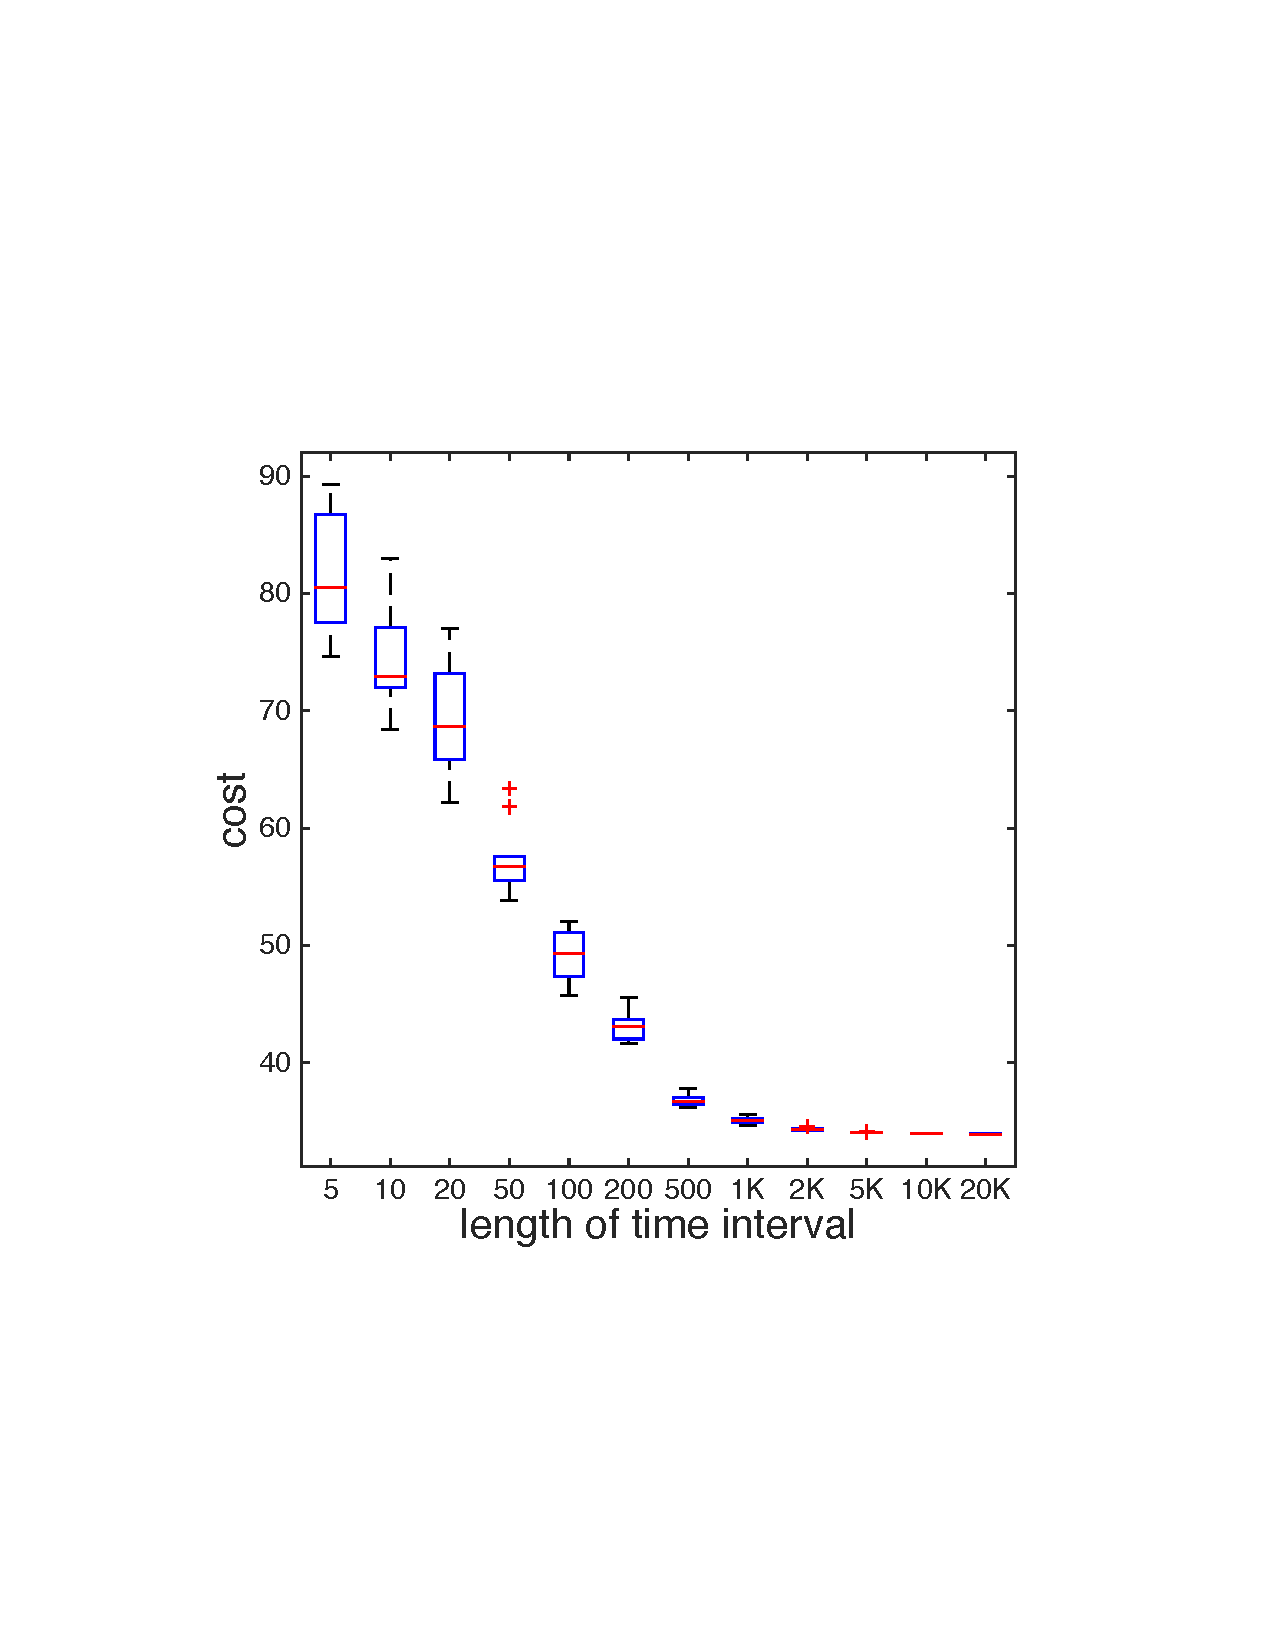
\includegraphics[width=0.49\textwidth]{figures/D100s/cost.pdf}}
	\subcaptionbox*{}{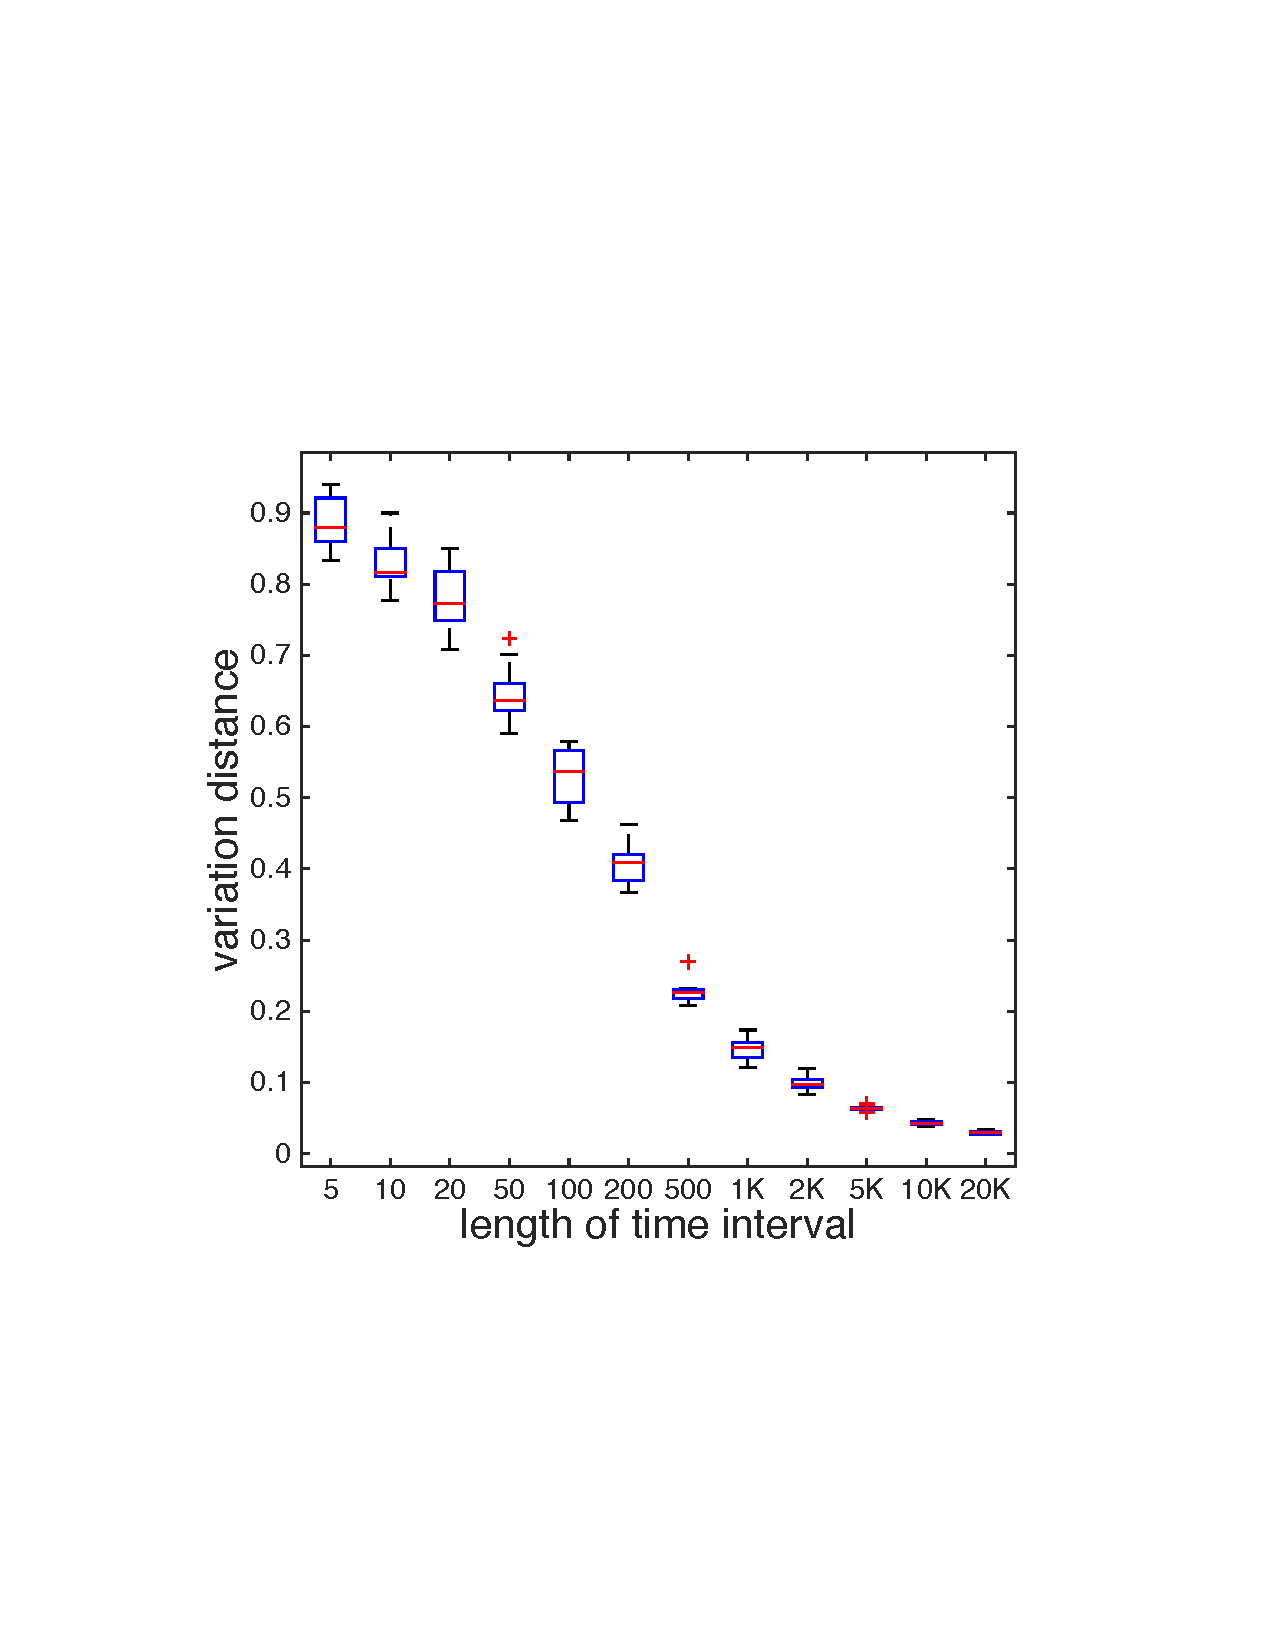
\includegraphics[width=0.49\textwidth]{figures/D100s/vardist.pdf}}
	\caption{\scriptsize The cost of \algonameapx outputs and their variation distance to the optimal schedule.} \label{fig:unique}
\end{figure}
In our experiments we run the \algonameapx algorithm, using (i) different \emph{random} initial schedules, and (ii) samples $\Sample$ obtained from time intervals of different lengths. For each sample, we run \algonameapx 10 times with 10 different random initial schedules, and compute the \textbf{exact} cost of each schedule, and its variation distance to the uniform schedule. Our results are plotted in Figure~\ref{fig:unique}, and as shown, by increasing the sample size (using longer time intervals of sampling) the output schedules gets very close to the uniform schedule (the variance gets smaller and smaller).

%-----------------------------------------------------------
%-----------------------------------------------------------
%-----------------------------------------------------------

\subsection{Dynamic Settings}\label{sec:dynset}
In this section, we present experimental results that show
 how our algorithm can adapt itself to the new situation.
Simulations are provided in Figure~\ref{figure:changes}: for each graph, we
start by following an 1-optimal schedule in the graph. At the beginning of each
``gray'' time interval, the labels of the nodes are permuted randomly, to impose
great disruptions in the system. Following that, at
the beginning of each ``green'' time interval our algorithm starts gathering
samples of $\sys$. Then, \algonameapx computes the schedule for the new sample, using 50 rounds of iterations, and starts probing. The length of each colored time
interval is $R = \frac{3(\log(n)+\log(2))}{\epsilon^2(1-\theta)}$, $\epsilon=0.5$, motivated by
Theorem~\ref{thm:approx_sample}.

%\todo[ahmad]{for $\epsilon=0.1$ and without making nodes generate up to 10: running}

%and other intervals (three time intervals before, between, and after the colored time intervals) have length $10R$. Also, for sake of illustration, we assumed at each time step each node $i$ may generated up to 10 items (each having a chance of $\pi_i$ to be generated). Thus, the number of generated items at each node is a binomial random variable with parameters 10 and $\pi$.
%Note that we start the generating process at time 0. Hence, during the first few time steps the load of the generating process increases.

Since the cost function is defined asymptotically (and explains the asymptotic behavior of the system in response to a schedule), in  Figure~\ref{figure:changes} we plot the load of the system $L_\theta(t)$ over the time (blue), and the \emph{average} load in the normal and perturbed time intervals (red). Based on this experiment, and as shown in Figure~\ref{figure:changes}, after adapting to the new schedule, the effect of the disruption caused by the perturbation disappears immediately. Note that when the difference between the optimal cost and any other schedule is small (like web-Notredame), the jump in the load will be small (e.g. as shown in Figure~\ref{fig:conv}), the cost of the initial schedule for web-Notredame is very close the optimal cost (obtained after 30 iteration).

%Based on our experiments, shown in Figure~\ref{figure:changes}, we observe that (i) a sample gathered during a very short time interval suffices to minimize the load (and therefore the cost) of the generating process, and (ii) after adapting to the new schedule, the effect of the perturbation disappears immediately (see the Section~\ref{sec:dynamic} for theoretical upper bound). Finally, note that for each time $t$, we plot the loads $L_\theta(t)$, and not the cost function. This is because the load is what we can observe (which is a draw of random variables $L_\theta(t)$), as the cost function is the expected value of these random variables averaged over the time, and it explains  the asymptotic behavior of the system.



\begin{figure}
%  \centering
  \subcaptionbox*{}{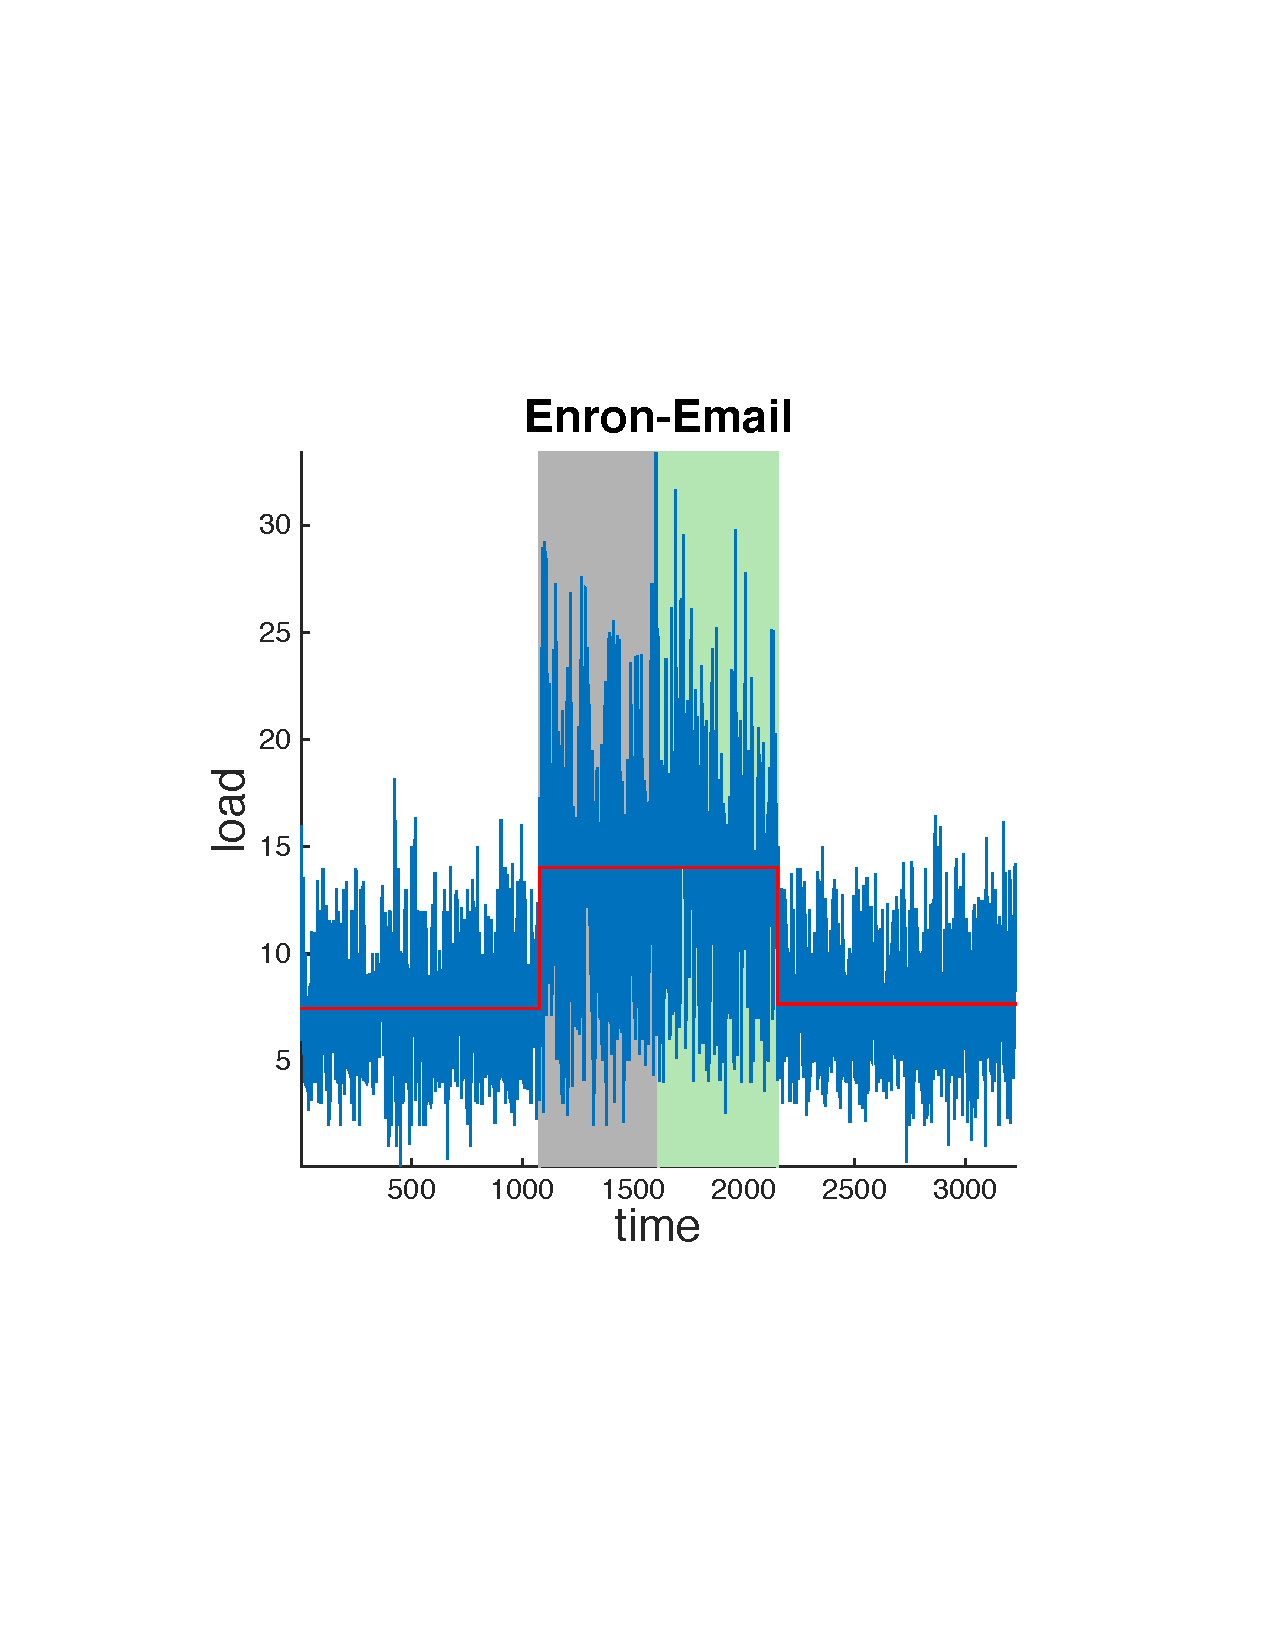
\includegraphics[width=0.49\textwidth]{figures/change/enron.pdf}} %\hspace{1em}%
  \subcaptionbox*{}{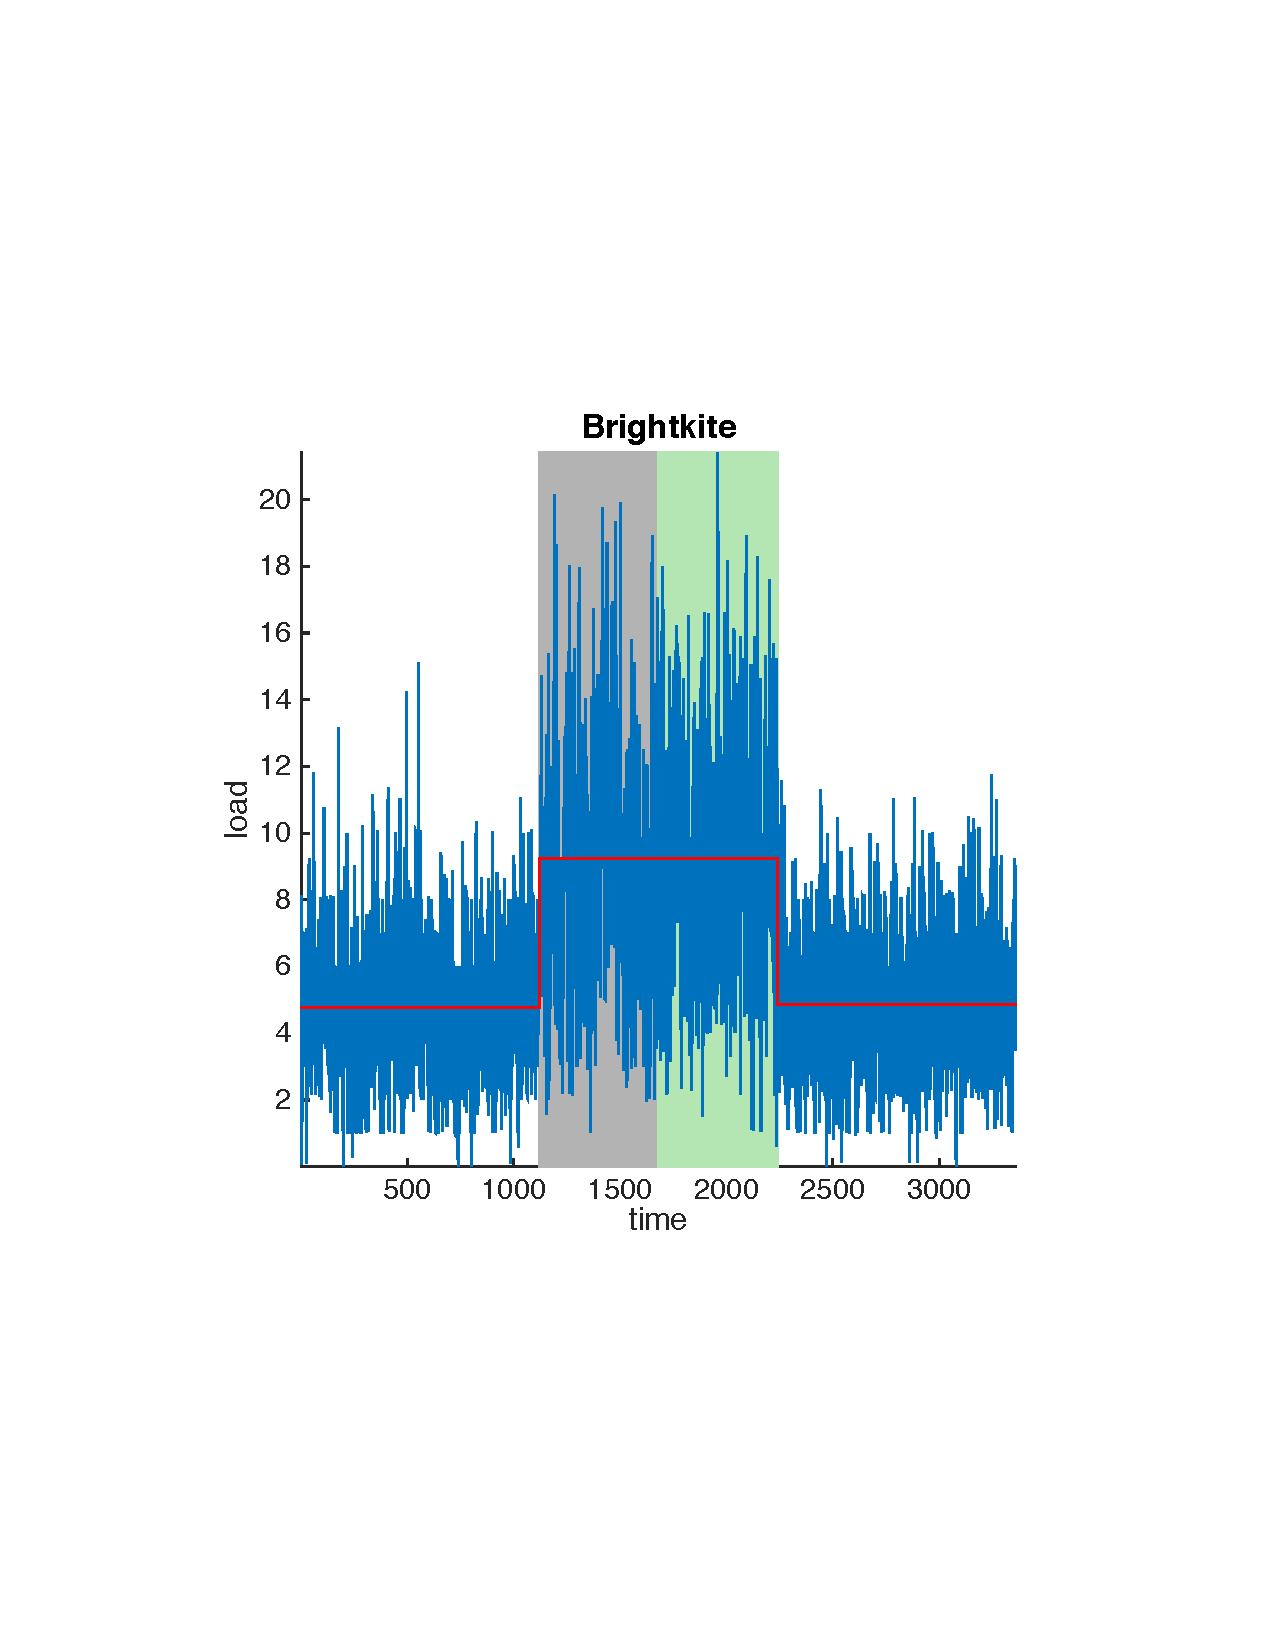
\includegraphics[width=0.49\textwidth]{figures/change/brightkite.pdf}} %\hspace{1em}
%  \subcaptionbox{Epinion\label{fig:change:epinion}}{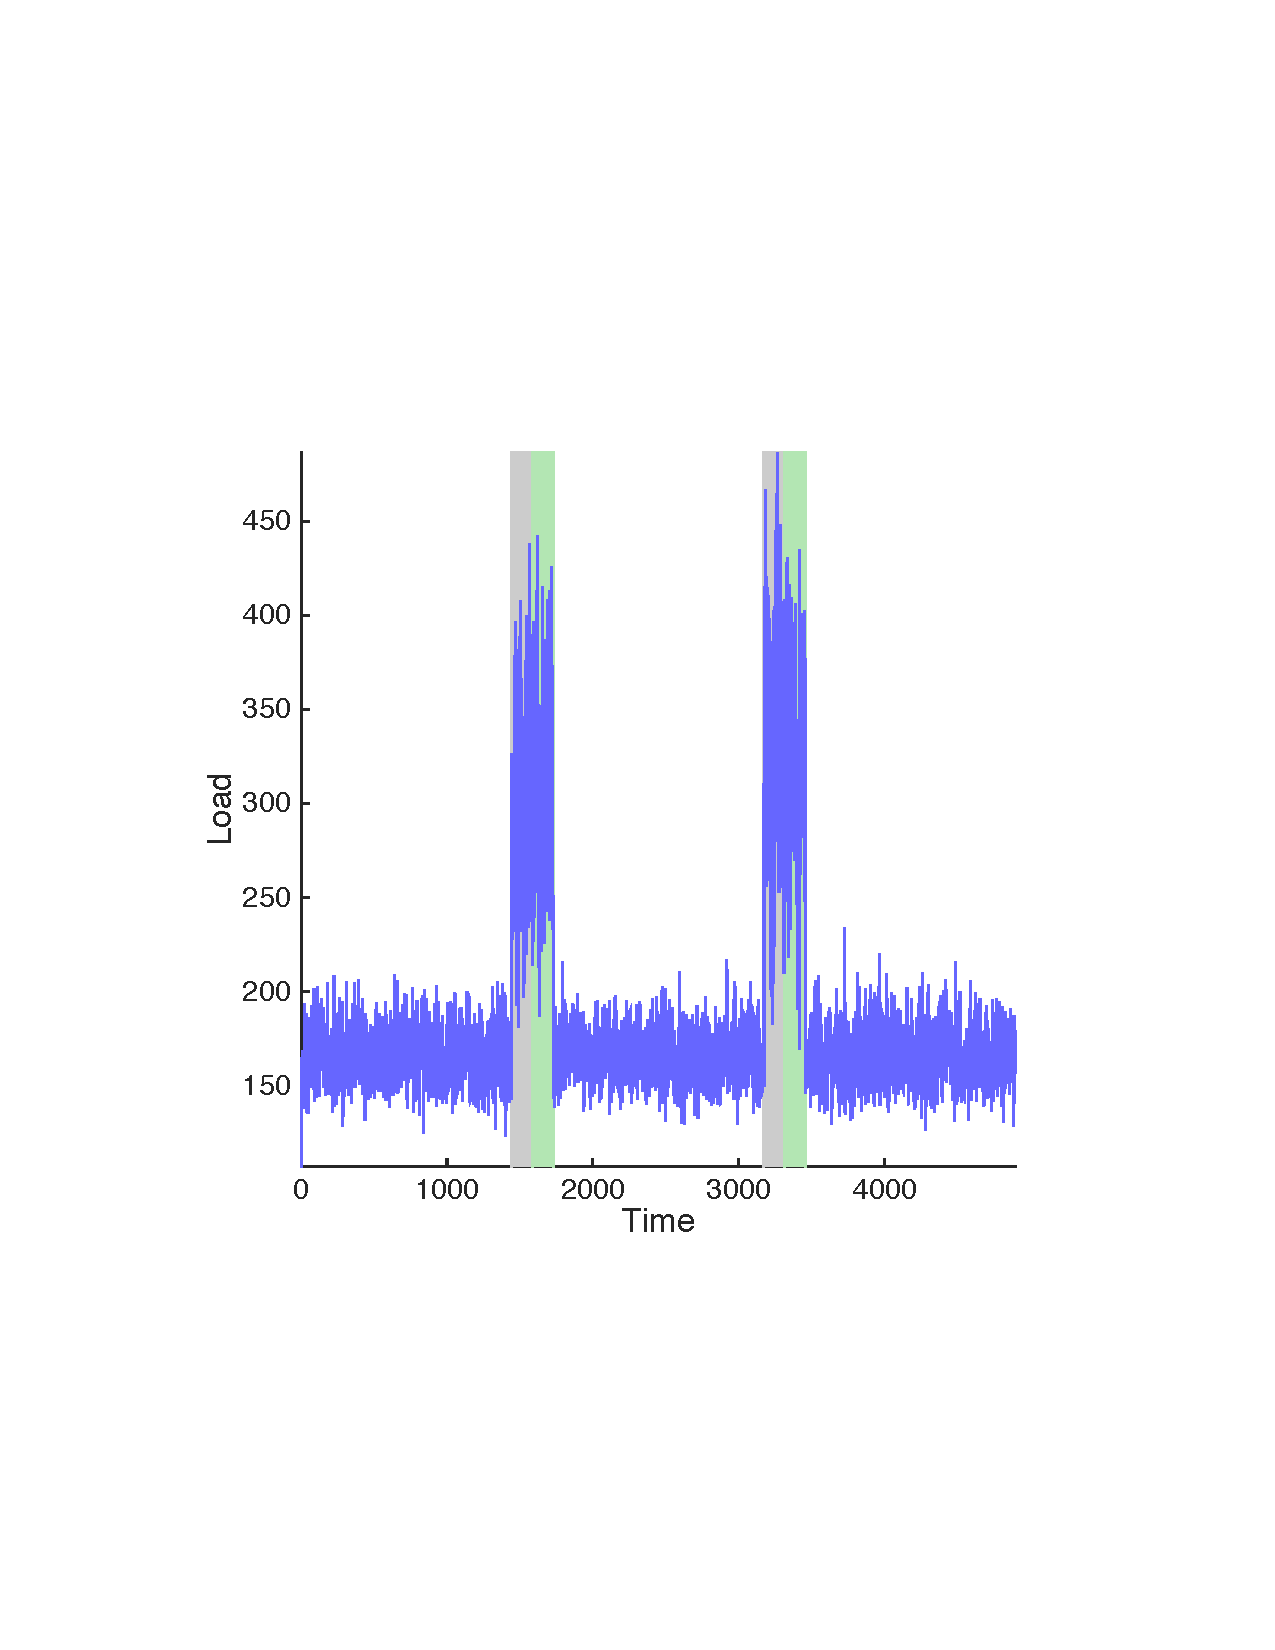
\includegraphics[width=0.3\textwidth]{figures/change/epinion.pdf}}\\ %\hspace{1em}\\
  \subcaptionbox*{}{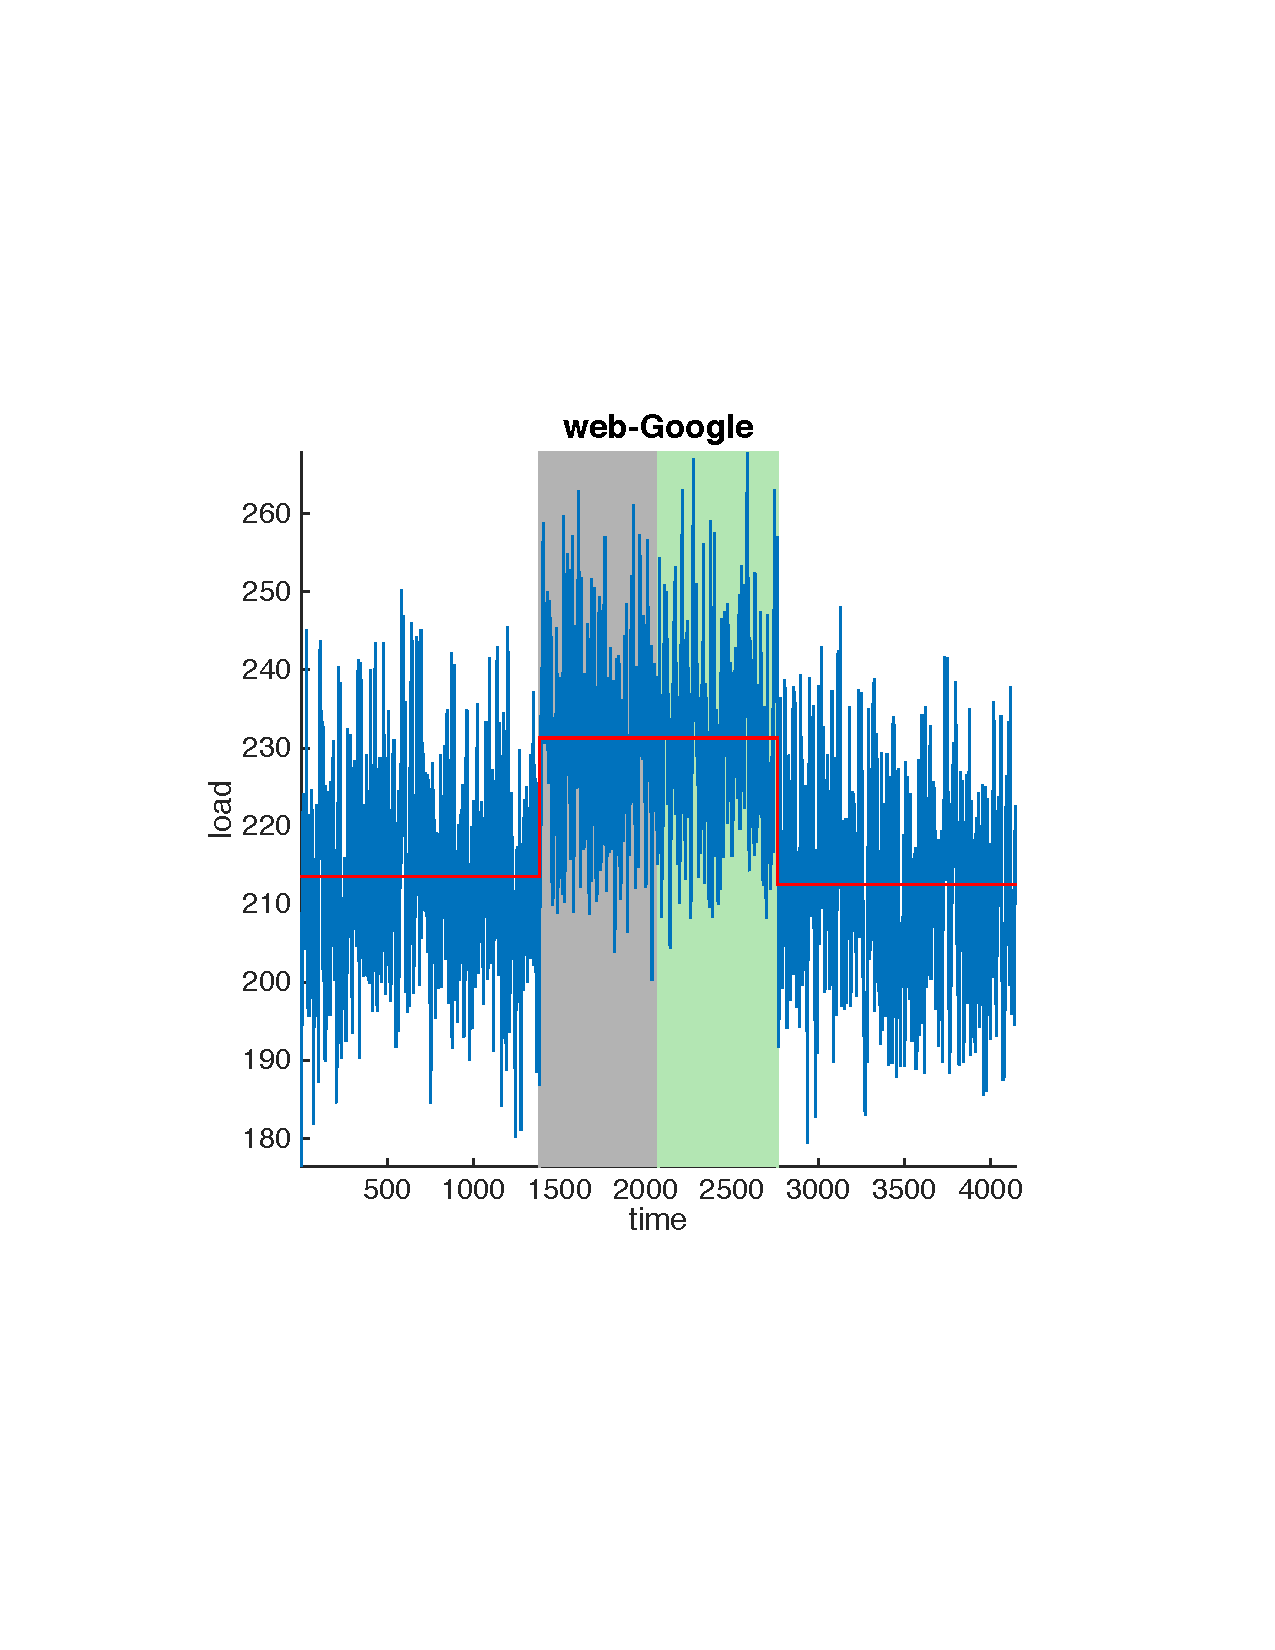
\includegraphics[width=0.49\textwidth]{figures/change/google.pdf}} %\hspace{1em}
  \subcaptionbox*{}{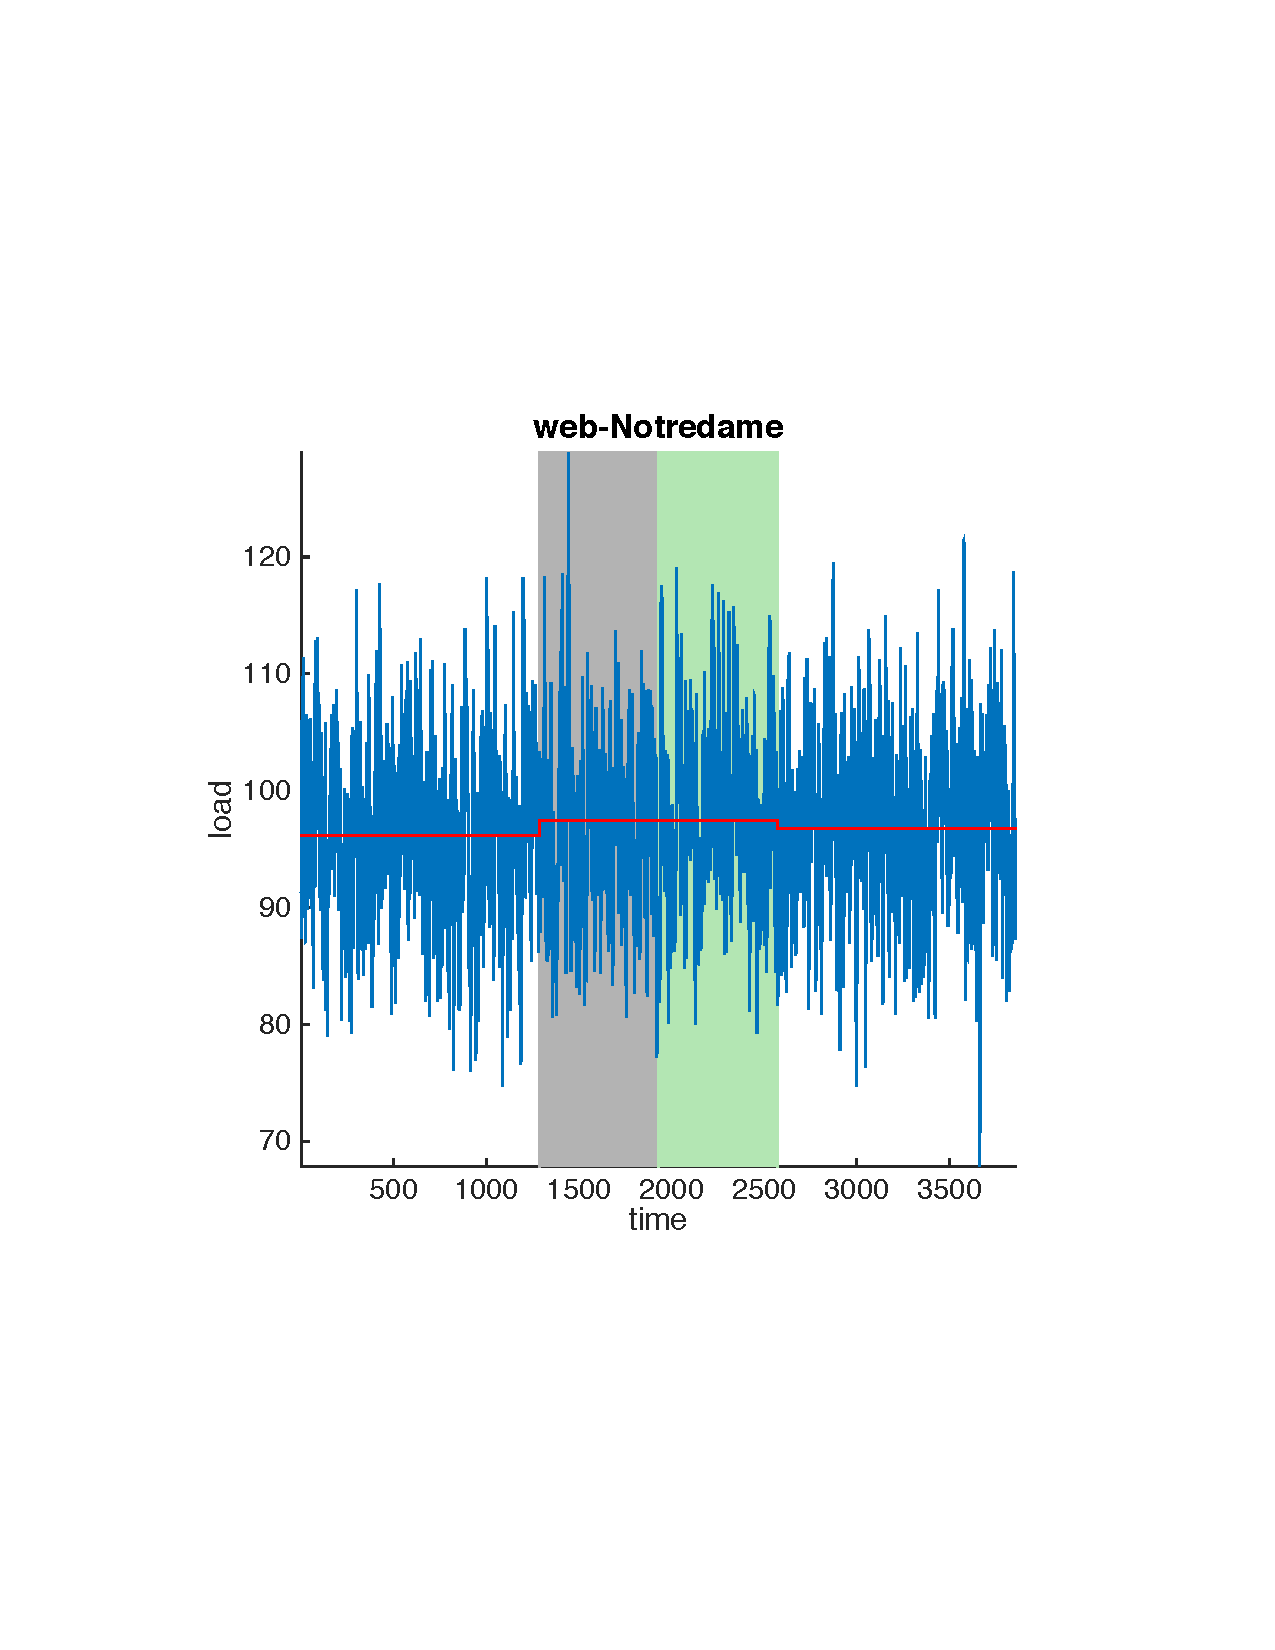
\includegraphics[width=0.49\textwidth]{figures/change/notredame.pdf}} %\hspace{1em}
  \caption{\scriptsize Perturbation, Sampling, and Adapting (For details see Section~\ref{sec:dynset}).}\label{figure:changes}
\end{figure}


